\section{Segnale di input}
% \begin{frame}
%   \begin{example}
%     \frametitle{Esempio di segnale di input.}
%       \begin{center}
%       \begin{figure}
% 	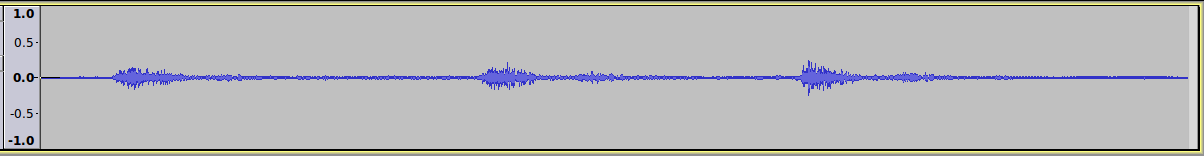
\includegraphics[width=0.9\textwidth]{./normal.png}
% 	% normal.png: 1366x768 pixel, 72dpi, 48.19x27.09 cm, bb=0 0 1366 768
%       \end{figure}
%       \end{center}
%     \movie[label=cells,width=4cm,height=0.5cm,poster,showcontrols,duration=13s]{}{normal.wav}
%   \end{example}
% \end{frame}


\begin{frame}
  \frametitle{Caratteristiche del segnale di input}
  \framesubtitle{Sorgenti sonore del segnale}
  
  \begin{center}
    \begin{tikzpicture}    [->,>=stealth',shorten >=1pt,auto,node distance=3cm,
      thick,main node/.style={circle,fill=blue!20,draw,font=\sffamily\Large\bfseries}]
    %   [scale=.8,auto=left,every node/.style={fill=blue!20}]
%       \node (sorgente) at (0,2.625) {sorgente};
    
      \node (interna) at (0,1) 		{interna al corpo};
      \node (esterna) at (0,4.25) 	{esterna al corpo};
    
      \node (respiratoria) at (4.8,0.5) 		{respiratoria};
      \node (gastrointestinale) at  (5,0)	{gastrointestinale};
      \node (deglutitoria) at (5,1) 		{deglutitoria};
      \node (vocale) at (4.4,1.5) 		{vocale};
      \node (cardiocircolatoria) at (5,2) 	{cardiocircolatoria};
    
      \node (vdots) at (3.6,3.5) 	{$\vdots$};
      \node (voci) at (5,4) 		{voci di persone};
      \node (traffico) at (5.1,4.5) 	{traffico veicolare};
      \node (movimento) at (4.4,5)	{movimento};
      
      \node (normale) at (8,0.25) 		{normale};
      \node (anormale) at (8,0.75) 		{anormale};



      \foreach \from/\to in {interna/respiratoria,interna/gastrointestinale,interna/deglutitoria,interna/vocale,interna/cardiocircolatoria,
	  esterna/traffico,esterna/voci,esterna/movimento,esterna/vdots,
	  respiratoria/normale, respiratoria/anormale}
	\draw (\from) -- (\to);
    
    \end{tikzpicture}
  \end{center}
\end{frame}


\begin{frame}[t]
  \frametitle{Caratteristiche del segnale di input\footnote{\emph{Breath Analysis of Respiratory Flow using Tracheal Sounds.} Saiful Huq, Azadeh Yadollahi, Zahra Moussavi. 2007 IEEE International Symposium on Signal Processing and Information Technology}}
  \framesubtitle{Valutazione sperimentale in assenza di rumore esterno}
\begin{center}
\begin{figure}
 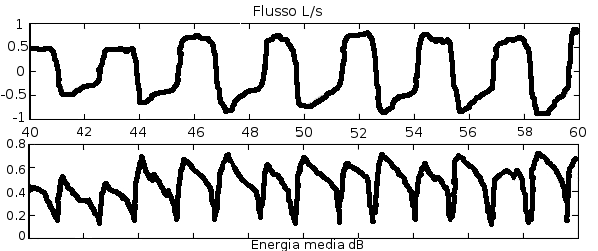
\includegraphics[width=\textwidth]{./ba2.png}
 % ba.png: 600x580 pixel, 72dpi, 21.16x20.46 cm, bb=0 0 600 580
\end{figure}
\end{center}
\end{frame}

% \begin{frame}
%   \frametitle{Caratteristiche del segnale di input\footnote{\emph{Breath Analysis of Respiratory Flow using Tracheal Sounds.} Saiful Huq, Azadeh Yadollahi, Zahra Moussavi. 2007 IEEE International Symposium on Signal Processing and Information Technology}}
%   \framesubtitle{Valutazione sperimentale}
% 
% % e anche altri studi (alcuni dei quali citati nella tesi) che usano metodi simili e arrivano a conclusioni simili
% 
% \begin{tikzpicture}[<->,>=stealth',shorten >=1pt,auto,node distance=3cm,
%   thick,main node/.style={fill=none,font=\large\sffamily}]
% 
%   \node[main node] (1) at (0,0) {intensit\`a del suono respiratorio};
% %   \node[main node] (5) at (0,0) {filtrato};
% %   \node[main node] (6) at (0,0.25) {senza rumore};
%   \node[main node] (4) at (2,2) {flusso respiratorio}; % flusso di un solo vettore!
% %   \node[main node] (2) [above left  of=4] {spirometro};
% %   \node[main node] (3) [above right of=1] {microfono};
% 
% 
%   \draw[every node/.style={font=\sffamily\small}]
% %     (1) edge node [left] {direttamente proporzionale} (4)
%       (1) edge node [right] {proporzionale} (4);
% %   \draw[every node/.style={font=\sffamily\small}, ->]
% %       (3) edge node [left] {misura} (1)
% %       (2) edge node [right] {misura} (4);
% %         edge [bend right] node[left] {0.3} (2)
% %         edge [loop above] node {0.1} (1)
% %     (2) edge node [right] {0.4} (1)
% %         edge node {0.3} (4)
% %         edge [loop left] node {0.4} (2)
% %         edge [bend right] node[left] {0.1} (3)
% %     (3) edge node [right] {0.8} (2)
% %         edge [bend right] node[right] {0.2} (4)
% %     (4) edge node [left] {0.2} (3)
% %         edge [loop right] node {0.6} (4)
% %         edge [bend right] node[right] {0.2} (1);
% % ;
% \end{tikzpicture}

% In questo studio gli autori studiano le differenze che ci sono tra la fase inspiratoria e la fase espiratoria in due quantit\`a relative ad un segnale tracheale filtrato con un filtro passa banda. 
% Queste due quantit\`a sono la media e la varianza logaritmica dell'energia. 
% Lo studio usa uno spirometro con pneumotacografo per misurare il flusso. 
% Il flusso viene diviso in base al valore assoluto in: basso, medio, alto e molto alto. 
%\paragraph{input}
%       I dati presi in input sono delle registrazioni di suoni tracheali registrati su nove soggetti sani e non fumatori i quali non hanno mai avuto gravi malattie respiratorie. 
%       Inoltre lo studio aveva a disposizione anche il flusso d'aria registrato attraverso uno spirometro con pneumotacografo
%     \paragraph{algoritmo}
%       L'algoritmo ha due flussi di esecuzione indipendenti, il primo \`e il seguente:
%       \begin{enumerate}
% 	\item 
% 	  Filtro passa alto con frequenza di taglio di $70Hz$ per rimuovere il rumore a bassa frequenza.
% 	\item
% 	  Nelle fasi seguenti l'algoritmo considera solo le porzioni del suono registrate quando il segnale del flusso era al di sotto del $20\%$ del flusso medio o al di sopra del $20\%$ di esso.
% 	  Perch\'e in queste condizioni il suono tracheale si pu\`o considerare stazionario.
% 	\item
% 	  Lo spettro di potenza dei suoni della trachea \`e stato calcolato in una finestra di $50ms$ ($512$ campioni) con il $75\%$ di sovrapposizione tra finestre successive. 
% 	  Per ogni fase respiratoria durante la quale c'era un diverso flusso d'aria, \`e stata calcolata la media della potenza dei suoni tracheali in decibel  entro sei predefinite bande di frequenza: da $70$ a $300Hz$, da $300$ a $450Hz$, da $450$ a $600Hz$, da $600$ a $800Hz$, da $800$ a $1000Hz$ e da $1000$ a $1200Hz$. 
% 	\item
% 	  Dato che le intensit\`a dei suoni respiratori variano da soggetto a soggetto, per ogni soggetto i valori calcolati in precedenza sono stati normalizzati rispetto al valore massimo.
% 	\item
% 	  Si \`e poi calcolata la media dei valori normalizzati tra soggetti diversi per ogni fase respiratoria, inoltre sono state calcolate la media e l'errore standard per diversi tassi di flusso e intervalli di frequenza.
%       \end{enumerate} 
%       mentre il secondo flusso di esecuzione \`e:
%       \begin{enumerate}
% 	\item
% 	  Il segnale dei suoni della trachea sono stati filtrati attraverso un filtro passa alto nelle stesse frequenze menzionate in precedenza. 
% 	\item
% 	  Il segnale filtrato \`e stato in seguito segmentato in finestre di dimensione $50ms$ ($512$ campioni) con il $75\%$ di sovrapposizione tra finestre successive usando una finestra di Hanning. 
% 	\item
% 	  Si calcola il logaritmo della varianza dei segmenti precedenti.
% 	\item
% 	  In ciascuna finestra il valore precedente viene normalizzato rispetto al valore massimo per ridurre le interferenze dei suoni del cuore
% 	\item	
% 	  In seguito viene calcolata la media all'interno delle diverse bande di frequenza e diversi valori del flusso d'aria.
%       \end{enumerate}
%     
%     \paragraph{conclusioni}
%       % \begin{figure}
% 	%  \centering
% 	%  \includegraphics[width=0.9\textwidth]{../Dropbox/tesi respiro/articoli stato dell'arte 1/Breath Analysis of Respiratory Flow using Tracheal Sounds Figura.png}
% 	%  % Breath Analysis of Respiratory Flow using Tracheal Sounds Figura.png: 953x548 pixel, 72dpi, 33.62x19.33 cm, bb=0 0 953 548
% 	%   \label{baorfutsf}
% 	%   
%       % \end{figure}
%       % medium and high flow rate samples of the recorded flow signal along with the spectrogram of the corresponding tracheal sound signal, the normalized logvariance and the normalized Pave over [300-450] Hz.  
%       % It should be noted that the positive (negative) values of the recorded flow signal are related to the inspiratory (expiratory) phases of the respiration cycle. 
%       Da una analisi dello spettrogramma dei suoni tracheali, si pu\`o vedere che l'intensit\`a del suono tracheale aumenta con l'aumentare del valore assoluto del flusso. 
%       Inoltre anche la varianza logaritmica normalizzata e la media di potenza normalizzata seguono i cambiamenti nel valore assoluto del flusso. 
%       Nello spettrogramma, nella varianza logaritmica normalizzata e nella media normalizzata della potenza sono evidenti le transizioni di fase respiratoria. 
%       Quando il flusso era medio o alto, si ha una maggiore differenza di media dell'energia normalizzata tra la fase inspiratoria ed espiratoria nella banda di frequenze dai $300$ ai $450Hz$. 
%       Inoltre questa banda di frequenza ottiene la seconda maggior differenza di media dell'energia normalizzata tra la fase inspiratoria e la fase esipiratoria quando il flusso \`e basso o molto alto. 
%       Quindi questo intervallo di frequenza \`e stato scelto come ottimale per esaminare i cambiamenti nella media della potenza rispettivamente alle fasi respiratorie.
% 
%   





% Lo tolgo questo frame?

% \begin{frame}
%    \frametitle{Caratteristiche del segnale di input}
%   \framesubtitle{Valutazione sperimentale 2}
% \begin{tikzpicture}[<->,>=stealth',shorten >=1pt,auto,node distance=3cm,
%   thick,main node/.style={fill=none,font=\sffamily}]
% 
%   \node[main node] (1) at (0,0.5) {varianza della dimensione};
%   \node[main node] (2) at (0,0.2) {frattale};
%   \node[main node] (3) at (7,0.5) {cambiamento di segno nel}; 
%   \node[main node] (4) at (7,0.2) {flusso respiratorio};
% 
% 
% 
%   \draw[every node/.style={font=\sffamily\small}]
% %     (1) edge node [left] {direttamente proporzionale} (4)
%       (1) edge node [above] {proporzionale} (3);
% %   \draw[every node/.style={font=\sffamily\small}, ->]
% %       (3) edge node [left] {misura} (1)
% %       (2) edge node [right] {misura} (4)
% %         edge [bend right] node[left] {0.3} (2)
% %         edge [loop above] node {0.1} (1)
% %     (2) edge node [right] {0.4} (1)
% %         edge node {0.3} (4)
% %         edge [loop left] node {0.4} (2)
% %         edge [bend right] node[left] {0.1} (3)
% %     (3) edge node [right] {0.8} (2)
% %         edge [bend right] node[right] {0.2} (4)
% %     (4) edge node [left] {0.2} (3)
% %         edge [loop right] node {0.6} (4)
% %         edge [bend right] node[right] {0.2} (1);
% % ;
% \end{tikzpicture}
% 
% \end{frame}





\begin{frame}
  \frametitle{Caratteristiche del segnale di input}
  \framesubtitle{Valutazione anatomico funzionale}
  \begin{itemize}
    \item Origine anatomico funzionale dei suoni respiratori
%     come vengono prodotti i suoni respiratori!!!
    \item Osservazione chiave:
      \textcolor{red}{L'apnea c'\`e quando il flusso \`e zero}
  \end{itemize}
\end{frame}


